\documentclass{article}
\usepackage[utf8]{inputenc}

\title{{\Huge Rapport de projet}}
\author{{\huge Equipe de projet 68 :} \\ {\LARGE Guillaume Bouchex-Bellomié, Loïc Broyer, } \\ \LARGE{Benoît Chahriar, Victor du Buat, Nathan Thirion}}
\date{{\large Mai 2019}}

\usepackage[french]{natbib}
\usepackage[french]{graphicx}
\usepackage[margin=0.5in]{geometry}
\usepackage[toc,page]{appendix}
\usepackage{amsmath} 

\renewcommand{\partname}{}

\begin{document}

\begin{flushleft}
 
\includegraphics[scale = 0.15]{logoPhelma}
\end{flushleft}
{\let\newpage\relax\maketitle}

\newpage
\null
\newpage

\renewcommand{\contentsname}{\Huge{Sommaire}}
\tableofcontents
\newpage
%Potentiellement mettre un glossaire et une liste des tableaux et images


\part{Introduction}
\section{Contexte}

Notre projet se développe en lien avec la participation du club Robotronik à l’édition 2019 de la coupe de France de robotique entre le 30 mai et le premier juin. Bien que tous les membres de notre équipe soient par ailleurs membres du club Robotronik, ce n’est pas en tant que tels que nous développons ce projet.
\newline\newline
Dans cette compétition, deux équipes disposant chacune de un ou deux robots doivent pousser des palets disposés sur le terrain et les ranger dans des cases. Les palets représentent des atomes auxquels une couleur est associé. Les cases sont des zones colorées du terrain placées sur une extrémité du terrain figurant un « tableau de Mendeleiev ». Par ailleurs, les robots peuvent également pousser un palet dans un couloir placé sur un des bords du terrain. Chacune de ces actions rapporte des points à l’équipe qui sont comptabilisés en fin de partie. Un espace libre est réservé aux équipes pour les dispositifs de leur choix en haut du terrain sur un rectangle de dimensions l*L et de hauteur h (fig. \ref{fig:terrain})\newline\newline
 Afin de pouvoir réaliser ces actions, il est impératif de pouvoir se déplacer précisément sur le terrain et donc de connaître sa position. Par ailleurs, il est impératif de savoir la position des palets pour se diriger. Jusque là, l’asservissement était assuré à l’aide d’encodeurs et le repérage des palets était réalisé en sondant l’environnement à l’aide de capteurs à ultrason disposés sur les robots. Le club Robotronik nous a commandé un système de repérage des palets et des robots basé sur le traitement d’images prises par une caméra placé en haut de l’espace réservé.
 
\begin{figure}[ht]
    \centering
    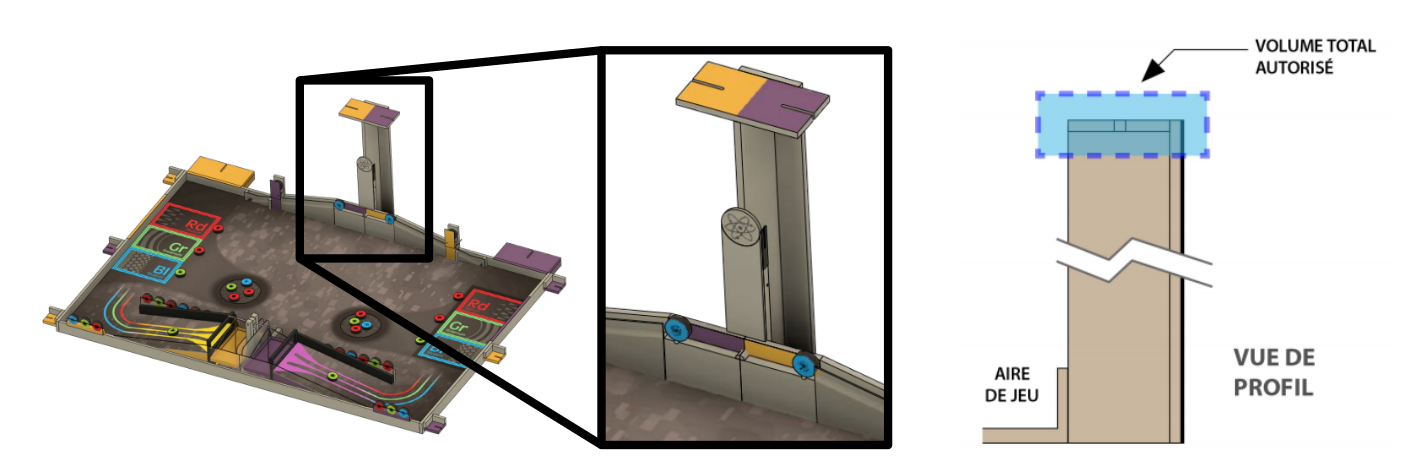
\includegraphics[scale = 0.3]{ImageTerrain}
    \caption{Représentation du terrain de jeu et de la zone utilisable pour notre projet}
    \label{fig:terrain}
\end{figure}

\section{Cadre de notre participation}

Ce projet nécessite de pouvoir acquérir des images du terrain, les analyser, et envoyer les données ainsi obtenues aux robots. Pour cela, il a fallu créer un support mécanique afin de pouvoir maintenir la caméra dans la même position souhaitée tout au long du match, acquérir les images, choisir le support du traitement et réaliser le logiciel l’exécutant, puis les modalités de communication.
\newline\newline
Le support mécanique doit respecter les règles de la coupe de France c'est à dire ne pas dépasser la position et les dimensions qui lui sont dédiées.
\newline\newline
La caméra est positionnée en hauteur sur une plateforme de 20cm sur 40cm partagée entre les deux équipes, laissant un espace disponible de 20cm sur 20cm pour le support. De plus, un dépassement de cet espace de 6cm est autorisé dans toutes les directions (fig. \ref{fig:terrain}) à l'exception de celle du support de l'autre équipe. La fixation à la plateforme se fait grâce à une fente de 8mm de diamètre au milieu de celle ci. Le support comportera donc un trou du même diamètre permettant d'y passer une vis serrée par un écrou papillon, maintenant le tout en place.
\newline\newline
Le support en lui même a été conçu pour accueillir une caméra Raspberry Pi et nous avons opté pour un modèle permettant de faire varier l'angle à volonté selon 2 axes (fig. \ref{fig:camera})

\begin{figure}[ht]
    \centering
    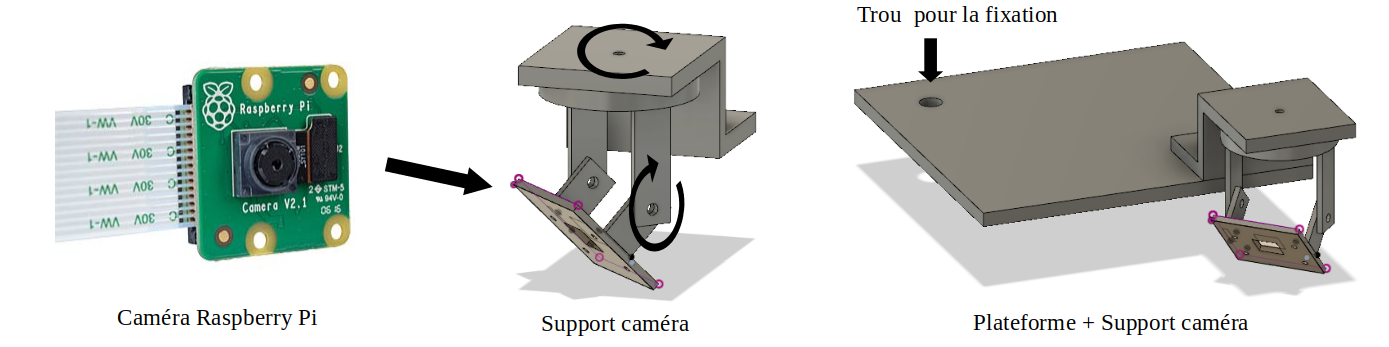
\includegraphics[scale = 0.3]{camera}
    \caption{Représentation du système d'attache de la caméra}
    \label{fig:camera}
\end{figure}

La caméra n'ayant pas un grand champs de vision, nous l'avons placée sur la plateforme afin qu'elle soit orientée principalement vers le coté du terrain dédié à notre équipe et le plus loin de celui ci. Par conséquent le support et la plateforme on été conçus pour pouvoir être séparés, car selon le côté alloué à notre équipe (que l'on ne peut pas prévoir), le montage doit être inversé pour regarder l'autre côté. Les deux axes de rotations peuvent êtres bloqués en serrant les vis des fixations. L'ensemble du montage à été conçu à l'aide du logiciel Fusion 360 de Autodesk et imprimé en 3D. Le reste de l'espace sur la plateforme sert à accueillir la Raspberry Pi en elle même. Nous avons pu tester notre prototype grâce à la réplique du terrain de la coupe de France fabriquée par l'association Robotronik.

\section{Division du travail et du projet}

\newpage
\part{Description de l'objectif}
\section{Cahier des charges}

\begin{tabular}{|l|c|c|}
\hline
\multicolumn{3}{|c|}{\bf \LARGE{Mécanique}}\\
\hline
\bf Fonction & \bf Critère & \bf Valeur\\
\hline
a & b & c\\
\hline
\hline
\multicolumn{3}{|c|}{\bf \LARGE{Matériel électronique}}\\
\hline
\bf Fonction & \bf Critère & \bf Valeur\\
\hline
Facilité de configuration du microprocesseur & b & c\\
\hline
Alimentation embarquée & Tension, courant & 5V, 3A\\
\hline
Possibilité de connexion de périphériques externes & b & c\\
\hline
Emettre un wifi local & b & c\\
\hline
Disponibilité de librairies et d'utilitaires & b & c\\
\hline
\hline
\multicolumn{3}{|c|}{\bf \LARGE{Informatique}}\\
\hline
\bf Fonction & \bf Critère & \bf Valeur\\
\hline
Lancement autonome des scripts au démarrage & b & c\\
\hline
Capacité à calculer l'orientation de la caméra & Précision angulaire & c\\
\hline
Capacité à convertir des coordonnées image en coordonnées physiques & Précision spatiale & c\\
\hline
\end{tabular}

\section{Description théorique}


\chapter{\bf \LARGE{Mécanique et matériel électronique}}

La Raspberry Pi est chargée avec une carte SD contenant toutes les librairies python utiles pour le projet (OpenCV, wifi, etc), ses codes bash et python.
Une caméra est branchée sur un port dédié de la carte et l'alimentation est reliée par un pin dédié sur la carte. Celle-ci est assurée par une batterie reliée à un régulateur de tension / courant permettant d'adapter la sortie de la batterie aux demandes de la Raspberry Pi.
En raison du fait qu'on n'aura pas beaucoup de temps ni d'écran lors de la Coupe de France de robotique pour tout mettre en place, la Raspberry Pi execute de manière automatique ses scripts de configuration et lance sa routine python quelques secondes après avoir été mise sous tension.
\newline\newline
\chapter{\bf \LARGE{Informatique}}

Le support mécanique de la caméra permettant d'obtenir une orientation variable sur deux axes, on doit être capable de déterminer avec précision les angles de la caméra par rapport au plan du terrain. Un code permet de determiner ces paramètres à partir de la connaissance des coordonnées physiques et sur l'image de deux points.
Ensuite, on est capable de relier les coordonnées sur l'image aux coordonnées physiques en fonction de la connaissance de la hauteur de la cible (robot ou palet). (Voir Annexe Théorique 1)
\newline\newline
Un point d'accès wifi indépendant a été préconfiguré sur la Raspberry Pi et est activé dès que la Raspberry Pi a terminé son chargement. Celui-ci n'est pas sécurisé car cela impliquerait plus de complexité et la sécurité n'est pas nécessaire pour les applications envisagées.
A la fin de chaque boucle d'execution du programme principal, les données relatives aux positions des robots et des palets sont envoyées sur le réseau. On pourra également envoyer directement l'image de la caméra (brute ou modifiée) pour débuguer en l'absence d'écran.

\newpage
\part{Mécanique et matériel}
\section{Impression 3D}
\section{Matériel électronique}

On a directement envisagé l'utilisation d'une Raspberry Pi pour effectuer toutes les opérations en raison du fait qu'elle permette d'intégrer un OS complet contrairement aux autres cartes (Arduino, STM32, etc). Ceci permet d'avoir déjà à disposition la librairie graphique OpenCV, l'interpréteur Python et d'autres utilitaires tel que le wifi. De plus, elle intègre un port dédié pour une caméra avec son logiciel. Nous avons priviligié l'utilisation de Raspbian comme OS en raison du fait qu'il intègre des pilotes dédiés pour la caméra.
Pour l'alimentation en période de développement, nous avions dans un premier temps envisagé d'utiliser un PC relié par USB, cependant cela ne satisfaisait pas les demandes en courant de la Raspberry Pi, aboutissant à des corruptions de la carte SD. Nous avons donc retenu l'alimentation par des chargeurs dédiés reliés à une prise électrique. Pour ce qui est de l'alimentation embarquée, nous avons prévu d'utiliser une batterie avec un régulateur de tension / courant.
\newline\newline
Sur la Raspberry Pi, on a réussi à compiler la librairie OpenCV utile au traitement d'image. Grâce à elle nous avons pu visualiser les images sortant de la caméra et nous assurer qu'elle fonctionnait bien.
Le lancement autonome des scripts prévus au démarrage a en revanche rencontré un problème. En effet, lorsque les commandes sont lancées depuis le terminal, tout fonctionne. Mais lorsque celles-ci sont executées depuis un script bash, on rencontre des erreurs. Nous nous contenterons de démarrer la Raspberry Pi en avance et de l'initialiser à la main si nous ne trouvons pas de solution à ce problème.

\newpage
\part{Informatique}
\section{Traitement de l'image}

\subsection{Modification de la perspective}
L'image filmée par la caméra est vue de côté, cette étape de traitement a pour but de tranformer l'image initiale en une vue de dessus.

\subsection{Détection de points de réference sur le terrain}
La modification du point de vue de l'image nécessite la détection, sur l'image initiale, de la position de points de reference. Les points dont on va chercher à 
détecter la position sur l'image ont été entourés sur la figure~\ref{image_init}.

La détection va être réalisée en deux étapes :
\begin{itemize}
\item détection du plus long côté du tableau périodique (entouré en noir sur la figure~\ref{3droites}), prise de ses deux extrémités, qui sont les points \no 1 et 2
\item détection des deux petits côtés (entourés en rouge), puis calcule des points \no 3 et 4.
\end{itemize}

\begin{figure}[!h]
   \begin{minipage}[t]{.46\linewidth}
      \begin{center}
      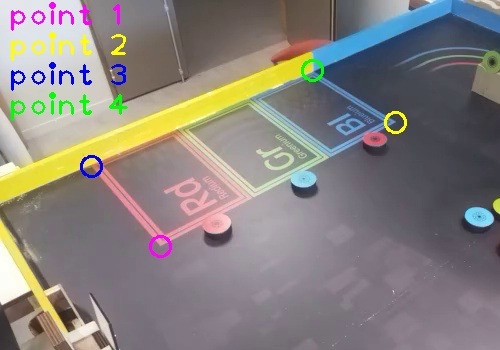
\includegraphics[height=150pt]{image_4_points.jpg}
      \end{center}
      \caption{Image filmée par la caméra du Raspberry Pi, les points recherchés ont été entourés}
      \label{image_init}
   \end{minipage} \hfill
   \begin{minipage}[t]{.46\linewidth}
      \begin{center}
      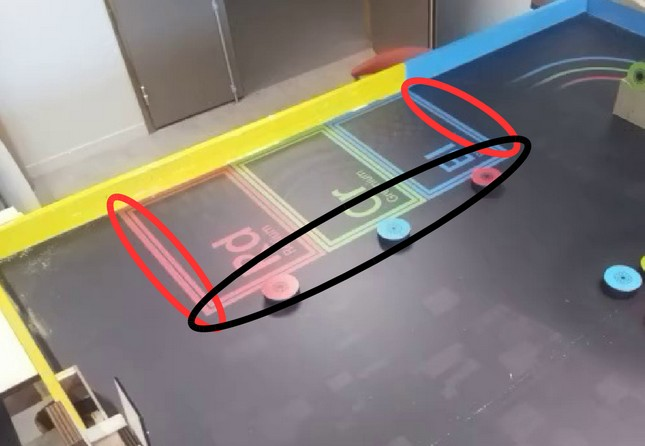
\includegraphics[height=150pt]{image_3_droites.jpg}
      \end{center}
      \caption{Les trois droites utilisées pour détecter les coins}
      \label{3droites}
   \end{minipage}
\end{figure}


\paragraph{Détection du long côté}
\subparagraph{Prise des contours}
L’application d’un filtre de Canny permet de mettre en évidence les contours présents dans l’image.
Le résultat de l’application de ce filtre est visible sur la figure~\ref{canny1}.
\begin{figure}[!h]
\begin{center} 
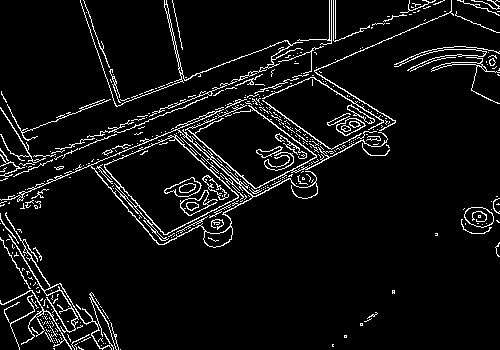
\includegraphics[height=130pt]{image_Canny.png}  
\end{center}
\caption{Résultat de l'application du filtre de Canny}
\label{canny1}
\end{figure}

\subparagraph{Détection de la droite}
La transformée de Hough détecte les droites présentes sur l’image. Cette fonction prend en argument un intervalle d’angle dans lequel rechercher des droites,
et le nombre minimum de pixels alignés pour qu’une droite soit détectée. Ces paramètres ont été choisi de manière à minimiser le nombre de droites détectées tout
en s’assurant que la droite recherchée ne soit pas ignorée. Les droites détectées par la transformée de Hough ont été tracées sur la figure~\ref{hough1}.

On recherche dans ces droites celle qui est la plus éloignée du coin en haut à gauche de l’image, elle a été tracée en violet.
\begin{figure}[!h]
\begin{center}
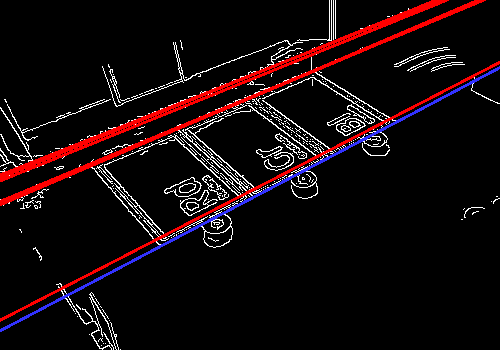
\includegraphics[height=130pt]{image_Canny_hough1.png}  
\end{center}
\caption{Résultat de la transformée de Hough, les droites détectés ont été tracés en rouge, et en bleu celle sélectionnée}
\label{hough1}
\end{figure}

\subparagraph{Détection des extrémités de cette droite}
La partie précédente a permis d’obtenir la droite recherchée, il faut maintenant en détecter les extrémités.

Un seuil de luminosité est appliqué à l’image initiale pour délimiter la zone du tableau périodique, sur la figure~\ref{seuillee} les pixels blancs
représentent les pixels de l’image ayant une luminosité suffisante. Pour une question de fiabilité, le seuil de luminosité qui est
appliqué n’est pas fixé par avance mais il est calculé à partir de la luminosité moyenne d’une partie de l’image où seul le fond gris
du tapis de jeu est visible.
Une opération « et logique » est ensuite appliquée entre la droite précédemment détectée et le résultat de l’opération de seuillage,
le résultat est donné sur la figure~\ref{droite1}. On récupère alors le plus long segment de cette image et on calcule la position de ses extrémités.

Cette première étape a permis de détecter deux coins du tableau périodique (les points 1 et 2 sur la figure~\ref{image_init}), ces points vont
faciliter la détection des deux petits côtés (encerclés en rouge sur la figure~\ref{3droites}).
\begin{figure}[!h] \hfill
   \begin{minipage}[t]{.4\linewidth}
      \begin{center}
      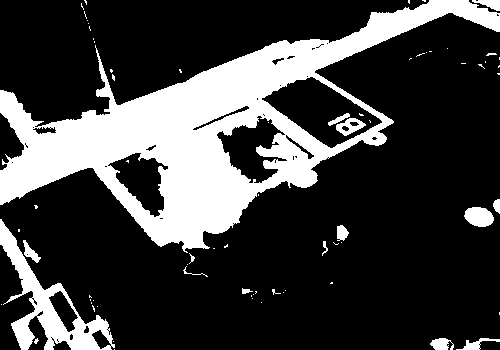
\includegraphics[height=130pt]{image_seuillee_en_luminosite.png}  
      \end{center}
      \caption{Image initiale seuillée en luminosité}
      \label{seuillee}
   \end{minipage} \hfill
   \begin{minipage}[t]{.4\linewidth}
      \begin{center}
      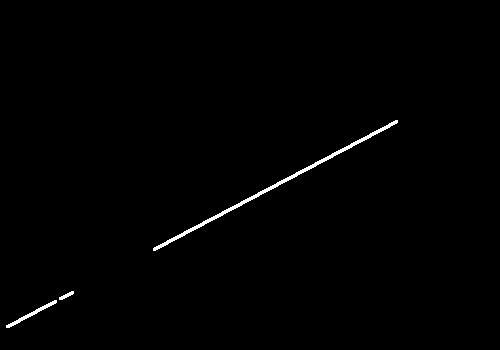
\includegraphics[height=130pt]{image_droite_1.png}  
      \end{center}
      \caption{Résultat de l'opération ``et logique'' entre l'image seuillée et la droite détectée}
      \label{droite1}
   \end{minipage} \hfill \hfill
\end{figure}

\paragraph{Détection des deux petits côtés}
\subparagraph{Détection de droites}
La transformée de Hough est à nouveau appliquée à l’image passée au filtre de Canny, avec des paramètres adaptés pour
les droites recherchées (voir figure~\ref{hough2}).
Pour chacun des points, on récupère la droite passant au plus près d’eux.
\begin{figure}[!h] \hfill
  \begin{minipage}[t]{.4\linewidth}
    \begin{center}
    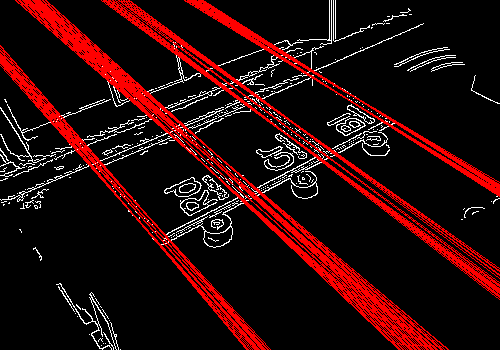
\includegraphics[height=130pt]{image_Canny_et_hough2.png}  
    \end{center}
    \caption{Résultat de la transformée de Hough}
    \label{hough2}
  \end{minipage} \hfill
  \begin{minipage}[t]{.4\linewidth}
    \begin{center}
    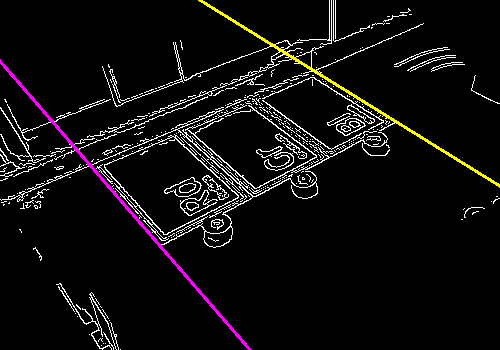
\includegraphics[height=130pt]{image_Canny_hough2_et_droites_choisies.png}  
    \end{center}
    \caption{Droites passant le plus près des deux points}
    \label{hough2bis}
  \end{minipage} \hfill\hfill
\end{figure}

\subparagraph{Calcul de la position des points \no3 et 4}
Les deux droites qui viennent d’être détectées donnent la direction du point \no1 vers le point 3, et du point \no2 vers le point 4,
on peut donc en déduire la position des points \no3 et 4

\subsection{Calcul d'une matrice de transformation de la perspective}
La position des points de reference obtenus précedemment va permettre de modifier le point de vue des images.

Une matrice de transformation de perspective est calculée telle que les quatre points sur l'image initiale se retrouvent
où ils seraient si le plateau de jeu avait été filmé en vue de dessus. En pratique, cette matrice est calculée pour que les points \no1 à 4
présent sur l'image de gauche de la figure~\ref{modif_perspective}, se retrouve aux points \no1' à 4' de l'image de droite.

\begin{figure}[!h]
\begin{center}
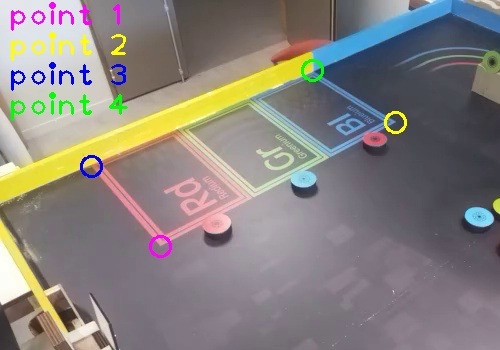
\includegraphics[height=130pt]{image_4_points.jpg}
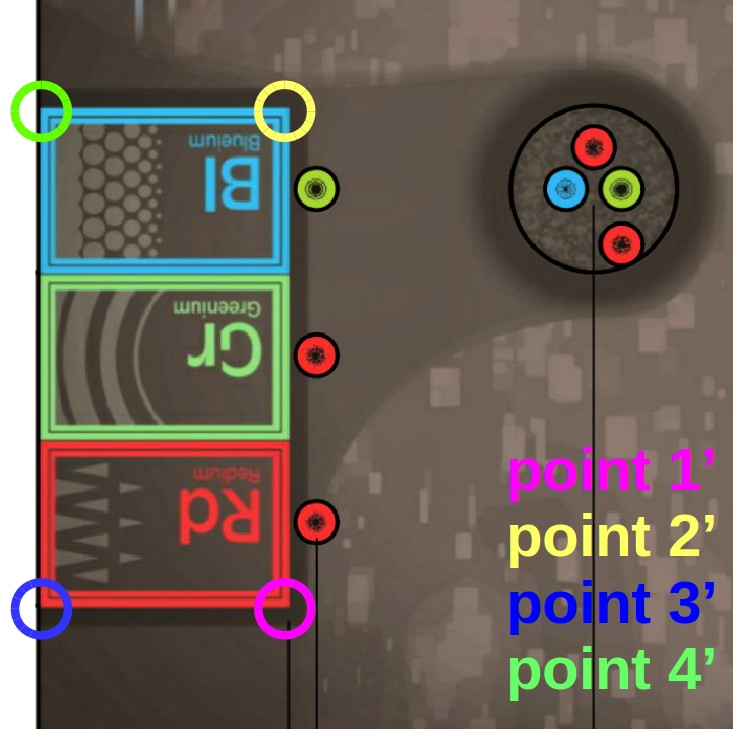
\includegraphics[height=130pt]{modif_perspective.jpg}
\end{center}
\caption{À gauche points détectés sur l'image initiale, à droite points d'arrivées entourés sur un schéma extrait du règlement de la coupe de France}
\label{modif_perspective}
\end{figure}

Cette matrice est ensuite appliquée à l'image intiale, le résultat est visible en figure~\ref{perspective_corrigee}

\begin{figure}[!h]
\begin{center}
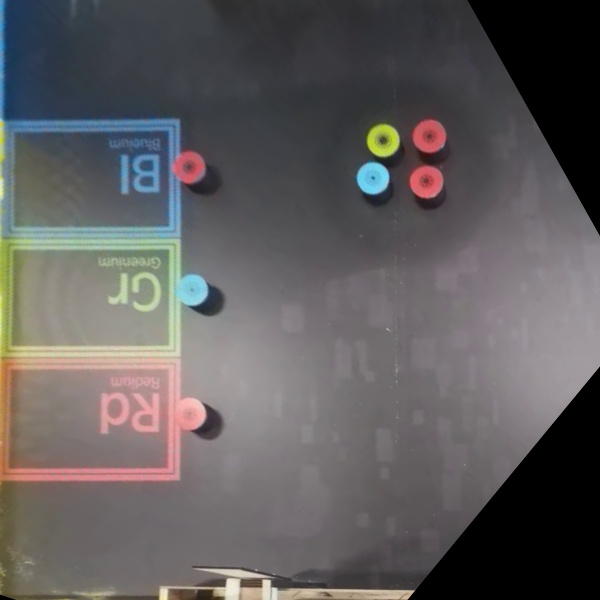
\includegraphics[height=150pt]{apres_modif_perspective.jpg}
\end{center}
\caption{Résultat de l'opération de modification de la perspective appliquée à l'image issue de la caméra}
\label{perspective_corrigee}
\end{figure}

\section{Détermination de la couleur des palets}
Afin de faciliter la détection des palets, leur couleur exacte est déterminée à partir de l'image initiale.
Les trois couleurs de palets (rouge, vert et bleu) sont les mêmes que les trois cases du tableau périodique, c'est donc la couleur des ces cases
qui est extraite car leur position est connue.

\paragraph{Extraction d'un échantillon de la couleur de chaque case du tableau périodique}
Les points \no1 et 2 sont utilisés pour extraire trois petites images contenant chacune une seule couleur.
L'échantillon de couleur rouge est extrait au voisinage du point \no1, celui de couleur bleue au voisinage du point \no2
et l'échantillon de couleur verte est extrait au voisinage du milieu du segment reliant les deux points.
Ces échantillons sont visible en figure~\ref{couleurs}.

\begin{figure}[!h]
\begin{center}
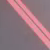
\includegraphics[height=70pt]{rouge_init.png}

\includegraphics[height=35pt]{vert_init.png}

\includegraphics[height=70pt]{bleu_init.png}
\end{center}
\caption{Échantillon des trois couleurs de palets}
\label{couleurs}
\end{figure}

\paragraph{Calcule de la valeur moyenne de couleur de chaque image}
Pour ces trois images, un seuillage en luminosité est appliqué afin de ne conserver que les pixels suffisamment lumineux.
Les pixels qui ne seront pas utilisés pour calculer la valeur moyenne de couleur ont été remplacés par des pixels noirs.
La valeur moyenne de couleur des pixels restants est calculée pour ces trois images.
\begin{figure}[!h]
\begin{center}
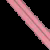
\includegraphics[height=70pt]{rouge_seuillee.png}

\includegraphics[height=35pt]{vert_seuillee.png}

\includegraphics[height=70pt]{bleu_seuillee.png}
\end{center}
\caption{Échantillon des trois couleurs de palets après seuillage}
\label{couleurs_seuillee}
\end{figure}

\section{Conversion de coordonnées}

En raison de la complexité des relations trigonométriques permettant de retrouver les angles en fonction de points sur l'image et sur le terrain, on exprime un angle en fonction de l'autre puis on utilise une procédure itérative de recherche du minimum de distance entre la position calculée et la position réelle. On a d'abord utilisé une résolution au centième de radian, puis on est passé au millième de radian. En effet, bien qu'en théorie le minimum est unique, il existe de nombreux points très proches du minimum et étant donné la résolution limitée, on peut le manquer et trouver un pseudo minimum avec des angles qui donneront un résultat complètement faux pour une autre position sur l'image.
\newline
On a mesuré l'orientation de la caméra et pris une image avec. Puis on a effectué des tests sur douze points de l'image en mesurant physiquement leur position sur le terrain avec la résolution du centième de radian et du millième de radian. On a observé dans tous les dcas des angles différents au centième de radian et dans tous les cas les bons angles au millième de radian. On garde donc la résolution au millième de radian.
\newline\newline
Le code de conversion des coordonnées image vers les coordonnées physiques permet en théorie de déterminer totalement la position des cibles, à condition que la position et l'orientation de la caméra soit précisément connue. En pratique, on retrouve effectivement cette limitation, la précision des positions calculées étant très dépendante de la précision des mesures de la position de la caméra (celles-ci impactant également le code de détermination des angles). En général, on trouvait les positions à moins d'un centimètre près.

\section{Connexion Wifi}

La Raspberry Pi avec Raspbian offre de nombreux utilitaires pour le wifi, donc nous nous basons sur leur utilisation. Du côté client, nous avions dans un premier temps codé un script python permettant de recevoir des données, pensant utiliser une Raspberry Pi sur les robots. Mais pour des raisons techniques, nous n'utiliserons qu'un module wifi branché à une carte STM32 sur les robots et avons codé ceci différemment. Cependant, ceci ne concerne pas strictement le projet et nous nous contenterons du code client python ici.
\newline\newline
Le point d'accès wifi a été configuré avec succès pour se lancer au démarrage de la Raspberry Pi. De plus, un code permettant d'envoyer n'importe quel type d'objet python par wifi a été réalisé. Ainsi, nous avons pu nous assurer que tout fonctionnait bien en envoyant par wifi le flux vidéo de la caméra vers un PC distant. Cependant, nous avons pu constater une importante latence (de l'ordre de quelques secondes) entre la réception et la capture des images. On peut attribuer cela au volume des images envoyées et des tests sur des envois de données plus petites nous a donné raison.
Du point de vue des clients, nous n'avons pas de problème à connecter un PC au wifi. Pour connecter les robots avec leur module wifi, cela nécessite encore du travail, mais c'est hors sujet ici.
\newpage

\part{Conclusion}



\bibliographystyle{plain}
\bibliography{references}

\newpage
\renewcommand\appendixtocname{Annexes}
\renewcommand\appendixpagename{Annexes}
\begin{appendices}
\chapter{\LARGE{Annexe 1 : Description théorique de la conversion des coordonnées image vers les  coordonnées physiques}}
\newline\newline

Cette annexe a pour but d'expliquer les mathématiques derrière la conversion des coordonnées image vers les coordonnées réelles.
\newline
On considérera dans la suite la géométrie de la (REF) pour la position et l'orientation de la caméra.

On part d'une image avec des coordonnées exprimées en pixels, la position (0,0) étant en haut à gauche de l'image (REF). Il sera important dans la suite de considérer si l'image est retournée ou pas (la gauche de l'image correspondrait à la droite de la caméra).


On va chercher à convertir cette image en coordonnées pixel en coordonnées sur un plan image fictif. Pour cela, on supposera que la caméra se situe à une distance 1 du plan. Ainsi, la distance maximale au centre de la bijection de l'image sur le plan image est en $\tan(\beta_0)$ et $\tan(\gamma_0)$. Ainsi, on utilisera la conversion décrite par (\ref{conversion}).

\begin{equation}
\label{conversion}
\left\{
    \begin{array}{ll}
        x = \tan(\beta_0)(\frac{2u}{resoX}-1)\\
        z = \tan(\gamma_0)(\frac{2v}{resoY} -1)
    \end{array}
\right.
\end{equation}
resoX étant le nombre de pixels en x et resoY respectivement en y, u et v étant les coordonnées sur l'image.

On peut interpréter la position sur le plan image comme un vecteur directeur de direction à partir de la caméra. On veut convertir cette direction dans le repère de la table et non plus celui de la caméra. Pour cela on va effectuer deux rotations successives correspondant aux angles $\gamma_0$ et $\beta_0$ de la caméra (\ref{rotation}).

\begin{equation}
\label{rotation}
\vec{P_{rot}} =
\begin{pmatrix}
\cos(\omega) & \sin(\omega)\cos(\alpha) & \sin(\omega)\sin(\alpha) \\
\sin(\omega) & \cos(\omega)\cos(\alpha) & \cos(\omega)\sin(\alpha)\\
0 & \sin(\alpha) & \cos(\alpha)\\
\end{pmatrix}
\quad
\vec{P_{cam}}
\end{equation}

A présent que l'on connaît la direction dans le repère du plan de jeu, on va calculer le point d'intersection de la droite partant de la caméra dans la direction $\vec{P_{rot}}$ avec le plan situé à une hauteur $h$ de la caméra (Cette hauteur étant à adapter en fonction de la nature de la cible, robot ou palet). Ces coordonnées s'obtiennent selon \ref{intersection}.

\begin{equation}
\label{intersection}
\left\{
    \begin{array}{ll}
        x = h * \frac{P_{rotX}}{P_{rotZ}}\\
        y = h * \frac{P_{rotY}}{P_{rotZ}}
    \end{array}
\right.
\end{equation}

Il ne reste plus qu'à éventuellement tenir compte d'une translation de la caméra par rapport à l'origine fixée quelque part sur la table.



\end{appendices}

\newpage
\chapter{\Huge {Resumé}}

\chapter{\Huge {Abstract}}
\end{document}

